\section{2-layer NN}

For the sake of simplicity, we will use a binary classification. Thus, the cost function is:

$$\mathcal{L}(y, \widehat{y})=-[y\log(\widehat{y})+(1-y)\log(1-\widehat{y})]$$

We notice that the loss function decreases when $y \neq \widehat y$, which is expected as we want to penalize wrong classification.

Forward propagation (with derivatives)

\begin{center}
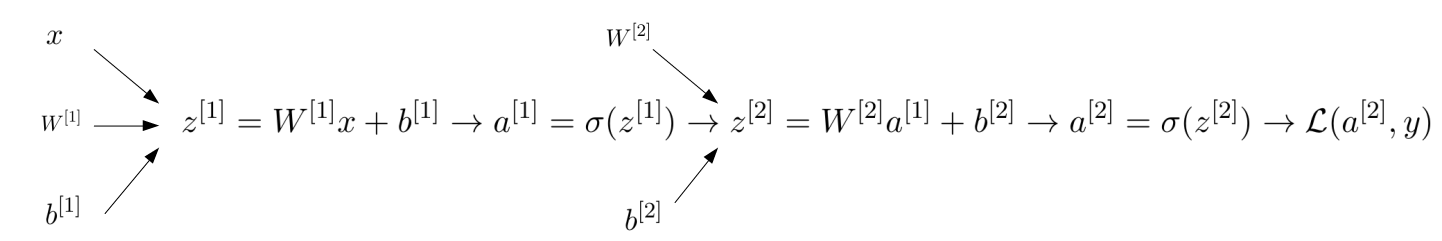
\includegraphics[scale=0.3]{img/NN_2.png}
\end{center}

As we can see here, we use two sets of weights and biases: $W^{[1]}$, $b^{[1]}$, $W^{[2]}$ and $b^{[2]}$. \\

Backward propagation (with derivatives)

\begin{center}
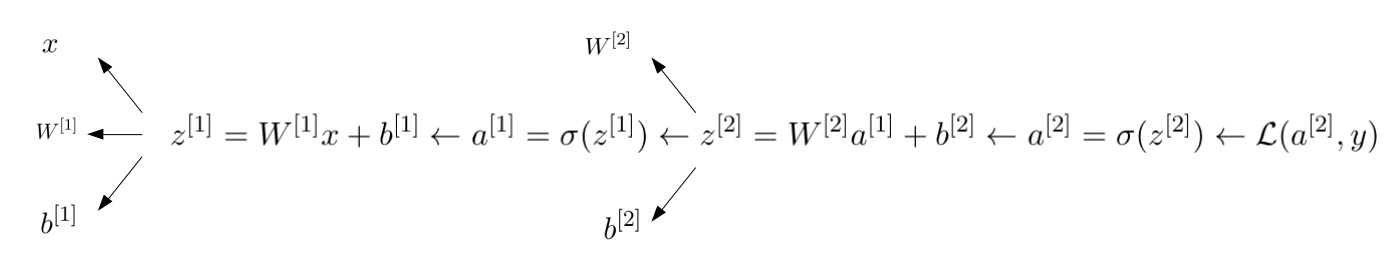
\includegraphics[scale=0.3]{img/NN_2_backward.png}
\end{center}

For the full details on the derivative computation, I explain everything on \href{https://github.savoga.io}{my website} (hopefully I didn't do too many mistakes).